\documentclass{article}

\usepackage{graphicx}
\usepackage{amsmath}
\usepackage[T5]{fontenc}
\usepackage[utf8]{inputenc}

% You can use a package 📦 called booktabs \usepackage{booktabs} for a visually better table.
\usepackage{booktabs}

\graphicspath{ {images/} }

% from begin-latex-in-minutes
\usepackage{listings}
\usepackage{color}

\lstdefinestyle{mystyle}{
keywordstyle=\color{magenta},
backgroundcolor=\color{yellow},
commentstyle=\color{green},
basicstyle=\footnotesize,
}
\lstset{style=mystyle}

\begin{document}

\begin{figure}[h]
    \centering
    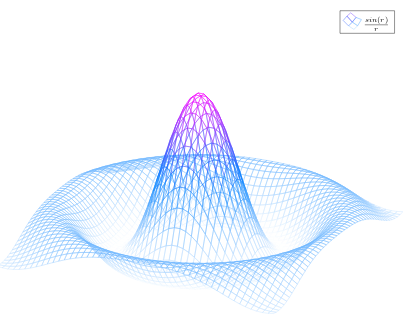
\includegraphics[width=0.25\textwidth]{mesh}
    \caption{a nice plot}
    \label{fig:mesh1}
\end{figure}

As you can see in the figure \ref{fig:mesh1}, the
function grows near 0. Also, in the page \pageref{fig:mesh1}
is the same example.

\begin{itemize}
  \item The individual entries are indicated with a black dot, a so-called bullet.
  \item The text in the entries may be of any length.
\end{itemize}

\begin{enumerate}
  \item This is the first entry in our list
  \item The list numbers increase with each entry we add
\end{enumerate}

In physics, the mass-energy equivalence is stated
by the equation $E=mc^2$, discovered in 1905 by Albert Einstein.

The mass-energy equivalence is described by the famous equation
\[ E=mc^2 \]
discovered in 1905 by Albert Einstein.
In natural units ($c = 1$), the formula expresses the identity
\begin{equation}
E=m
\end{equation}


Subscripts in math mode are written as $a_b$ and superscripts are written as $a^b$. These can be combined an nested to write expressions such as

\[ T^{i_1 i_2 \dots i_p}_{j_1 j_2 \dots j_q} = T(x^{i_1},\dots,x^{i_p},e_{j_1},\dots,e_{j_q}) \]

We write integrals using $\int$ and fractions using $\frac{a}{b}$. Limits are placed on integrals using superscripts and subscripts:

\[ \int_0^1 \frac{dx}{e^x} =  \frac{e-1}{e} \]

Lower case Greek letters are written as $\omega$ $\delta$ etc. while upper case Greek letters are written as $\Omega$ $\Delta$.

Mathematical operators are prefixed with a backslash as $\sin(\beta)$, $\cos(\alpha)$, $\log(x)$ etc.

\paragraph{dsfsfsdfds}
This is a paragraph. Hi let me introduce myself Hi let me introduce myself Hi let me introduce myself Hi let me introduce myself Hi let me introduce myself Hi let me introduce myself


\section{zczxzzcxzx}
We begin a section with section and a paragraph with paragraph. You can also add subsection with subsection and subparagraph with subparagraph

\subsection{zczxcxzcc}
We begin a section with section and a paragraph with paragraph. You can also add subsection with subsection and subparagraph with subparagraph
xcvcxvcxv

Hi let me introduce myself\footnote{\label{myfootnote}Hello footnote}.
... (later on)

I'm referring to myself \ref{myfootnote}.

\begin{table}[h!]
  \centering
  \caption{Caption for the table.}
  \label{tab:table1}

  \begin{tabular}{|l|c|||r|}
    \hline
    1 sadfsd sdfsf sfds & 2 sdfds dsfd sdf sdf & asdasd asd asdaad adaa 3\\
    \hline
    a & b xcv dfd dsf sdfsd & ada adsdc\\
    \hline
  \end{tabular}

\end{table}


\paragraph{dsfsfsdfds}
This is a paragraph. Hi let me introduce myself Hi let me introduce myself Hi let me introduce myself Hi let me introduce myself Hi let me introduce myself Hi let me introduce myself

\paragraph{dsfsfsdfds}
This is a paragraph. Hi let me introduce myself Hi let me introduce myself Hi let me introduce myself Hi let me introduce myself Hi let me introduce myself Hi let me introduce myself

\begin{figure}[h]
  % 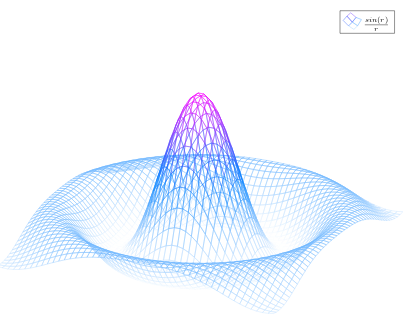
\includegraphics[width=\linewidth]{mesh.png}
  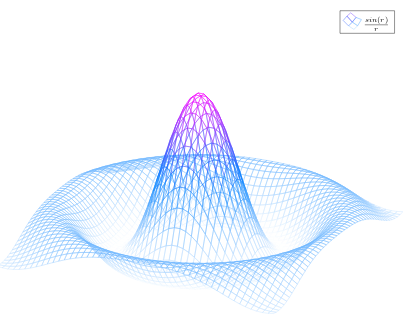
\includegraphics[width=0.25\linewidth]{mesh.png}
  \caption{What is it about?}
  \label{fig:whateverlabel}
\end{figure}

\begin{verbatim}
  #include <iostream>

  int main()
  {
    std::cout << "hello world!\n";
    return 0;
  }
\end{verbatim}

\begin{lstlisting}[language=Python]

  print "Hello World!"

\end{lstlisting}



Lorem ipsum dolor sit amet \lstinline{print "Hello World"} , consectetur adipiscing elit, sed do eiusmod tempor incididunt ut labore et dolore magna aliqua. Ut enim ad minim veniam, quis nostrud exercitation ullamco laboris nisi ut aliquip ex ea commodo consequat. Duis aute irure dolor in reprehenderit in voluptate velit esse cillum dolore eu fugiat nulla pariatur. Excepteur sint occaecat cupidatat non proident, sunt in culpa qui officia deserunt mollit anim id est laborum.

% part2.tex



\paragraph{!! test} test
Hello Latex, \par This is part2.tex dsfdddf

\indent sfsfsdfds sfsfsdfds

\indent
sfdsd sffdsf dsfsdf

\title{Company headquarters of}

\paragraph{!! Tips:}
For readability, clarity and maintenance purpose, it is highly suggested that you divide your
Main file systematically, hierarchically and scientifically.


Don't divide without reasons or you may get a mess later.




\end{document}